%% The following is a directive for TeXShop to indicate the main file
%%!TEX root = diss.tex

\chapter{Introduction}
\label{ch:Introduction}

%%%%%%%%%%%%%%%%%%%%%%%%%%%%%%%%%%%%%%%%%%%%%%%%%%%%%%%%%%%%%%%%%%%%%%
\section{The emergence of precision oncology}
\label{sec:Theemergenceofprecisiononcology}

Cancers are fundamentally a group of genetic disorders. The role of genetic alterations in driving malignant transformation has been implicated in studies dating back to the late nineteenth and early twentieth centuries by David von Hansemann and Theodor Boveri. Von Hansemann suggested that aberrant cell division accounted for unequal chromosome distributions in tumour cells \cite{VonHansemann1890, Paget2006}. Motivated by von Hansemann's findings, Boveri explored the outcomes of sea urchin embryos that were induced to divide abnormally. An intriguing observation that drew Boveri's attention was not all chromosomal imbalanced cells proliferated uncontrollably and formed tumours, there were some that resulted in cell death, thus indicating that genetic materials were functionally distinct. This led to Boveri's hypothesis that tumour development is promoted by retention of chromatin parts that stimulate growth or elimination of those that inhibit growth, concepts that manifested in the present-day knowledge of oncogenes and tumour-suppressor genes, respectively \cite{Boveri1914, Paget2006}.

Major strides have been made in understanding the molecular basis of cancer, including the discovery of recurrent gene mutations and elucidation of oncogenic pathways. Some of these findings have been successfully translated into clinical applications wherein patients who harbour actionable somatic mutations benefitted from treatment with targeted anti-cancer drugs. Notable examples include treatment of \acs{HER2}-overexpressed breast cancer with trastuzumab \cite{Slamon1987, Andrulis1998, Sjogren1998, Drebin1985, Vogel2002, Seidman2008}, \acs{BCR-ABL1}-translocated chronic myeloid leukemia with imatinib \cite{Rowley1973, Druker2006}, and \acs{BRAF}-mutated melanoma with vemurafenib \cite{Chapman2011, Ravnan2012}. The ability to improve clinical outcome by exploiting tumour genetic vulnerabilities has contributed to the advent of precision oncology, a framework that tailors patient care based on tumour genetic makeup.

As more actionable somatic mutations are revealed, precision oncology regimens begin to face limitations caused by single-gene assays, which pose challenges in scaling to meet diagnostic needs. Fortunately, these barriers have been surmounted by advances in next-generation sequencing (\acs{NGS}) technologies. By harnessing the high-throughput nature of NGS, traditional gene-by-gene approaches are being rapidly supplanted by targeted gene panels and genome-scale profiling, which surveys the whole exome or genome. The dramatic decline in sequencing cost \cite{Wetterstrand2016} and low requirement for DNA input \cite{Rykalina2014, Chung2016, So2017} have also accelerated the adoption of NGS-based genomic testing in clinical practice (\autoref{fig:cost_per_genome}). Furthermore, concurrent progress in algorithmic development has enabled efficient storage, processing, and interpretation of massive genomic data sets produced by NGS platforms \cite{Torri2012, Pabinger2014}. Automated variant analysis pipelines can be established by integrating these bioinformatics tools to allow accurate reporting of clinically significant genomic alterations \cite{Hyman2015, Laskin2015, Bosdet2013, Sheffield2016}. Hence, while the precision oncology framework has been instigated by the discovery of actionable somatic mutations, its translation into clinical use is largely catalyzed by advancements in \acs{DNA} sequencing technologies and analysis algorithms. Although research efforts are still underway in refining these technological components, it is undeniable that the precision oncology paradigm holds great potential in enhancing disease management and therapeutic intervention for cancer patients.

%%%%%%%%%%%%%%%%%%%%%%%%%%%%%%%%%%%%%%%%%%%%%%%%%%%%%%%%%%%%%%%%%%%%%
%%%%%%%%%%%%%%%%%%%%%%%%%%%%%%%%%%%%%%%%%%%%%%%%%%%%%%%%%%%%%%%%%%%%%

\begin{figure}[H]
	\centering
	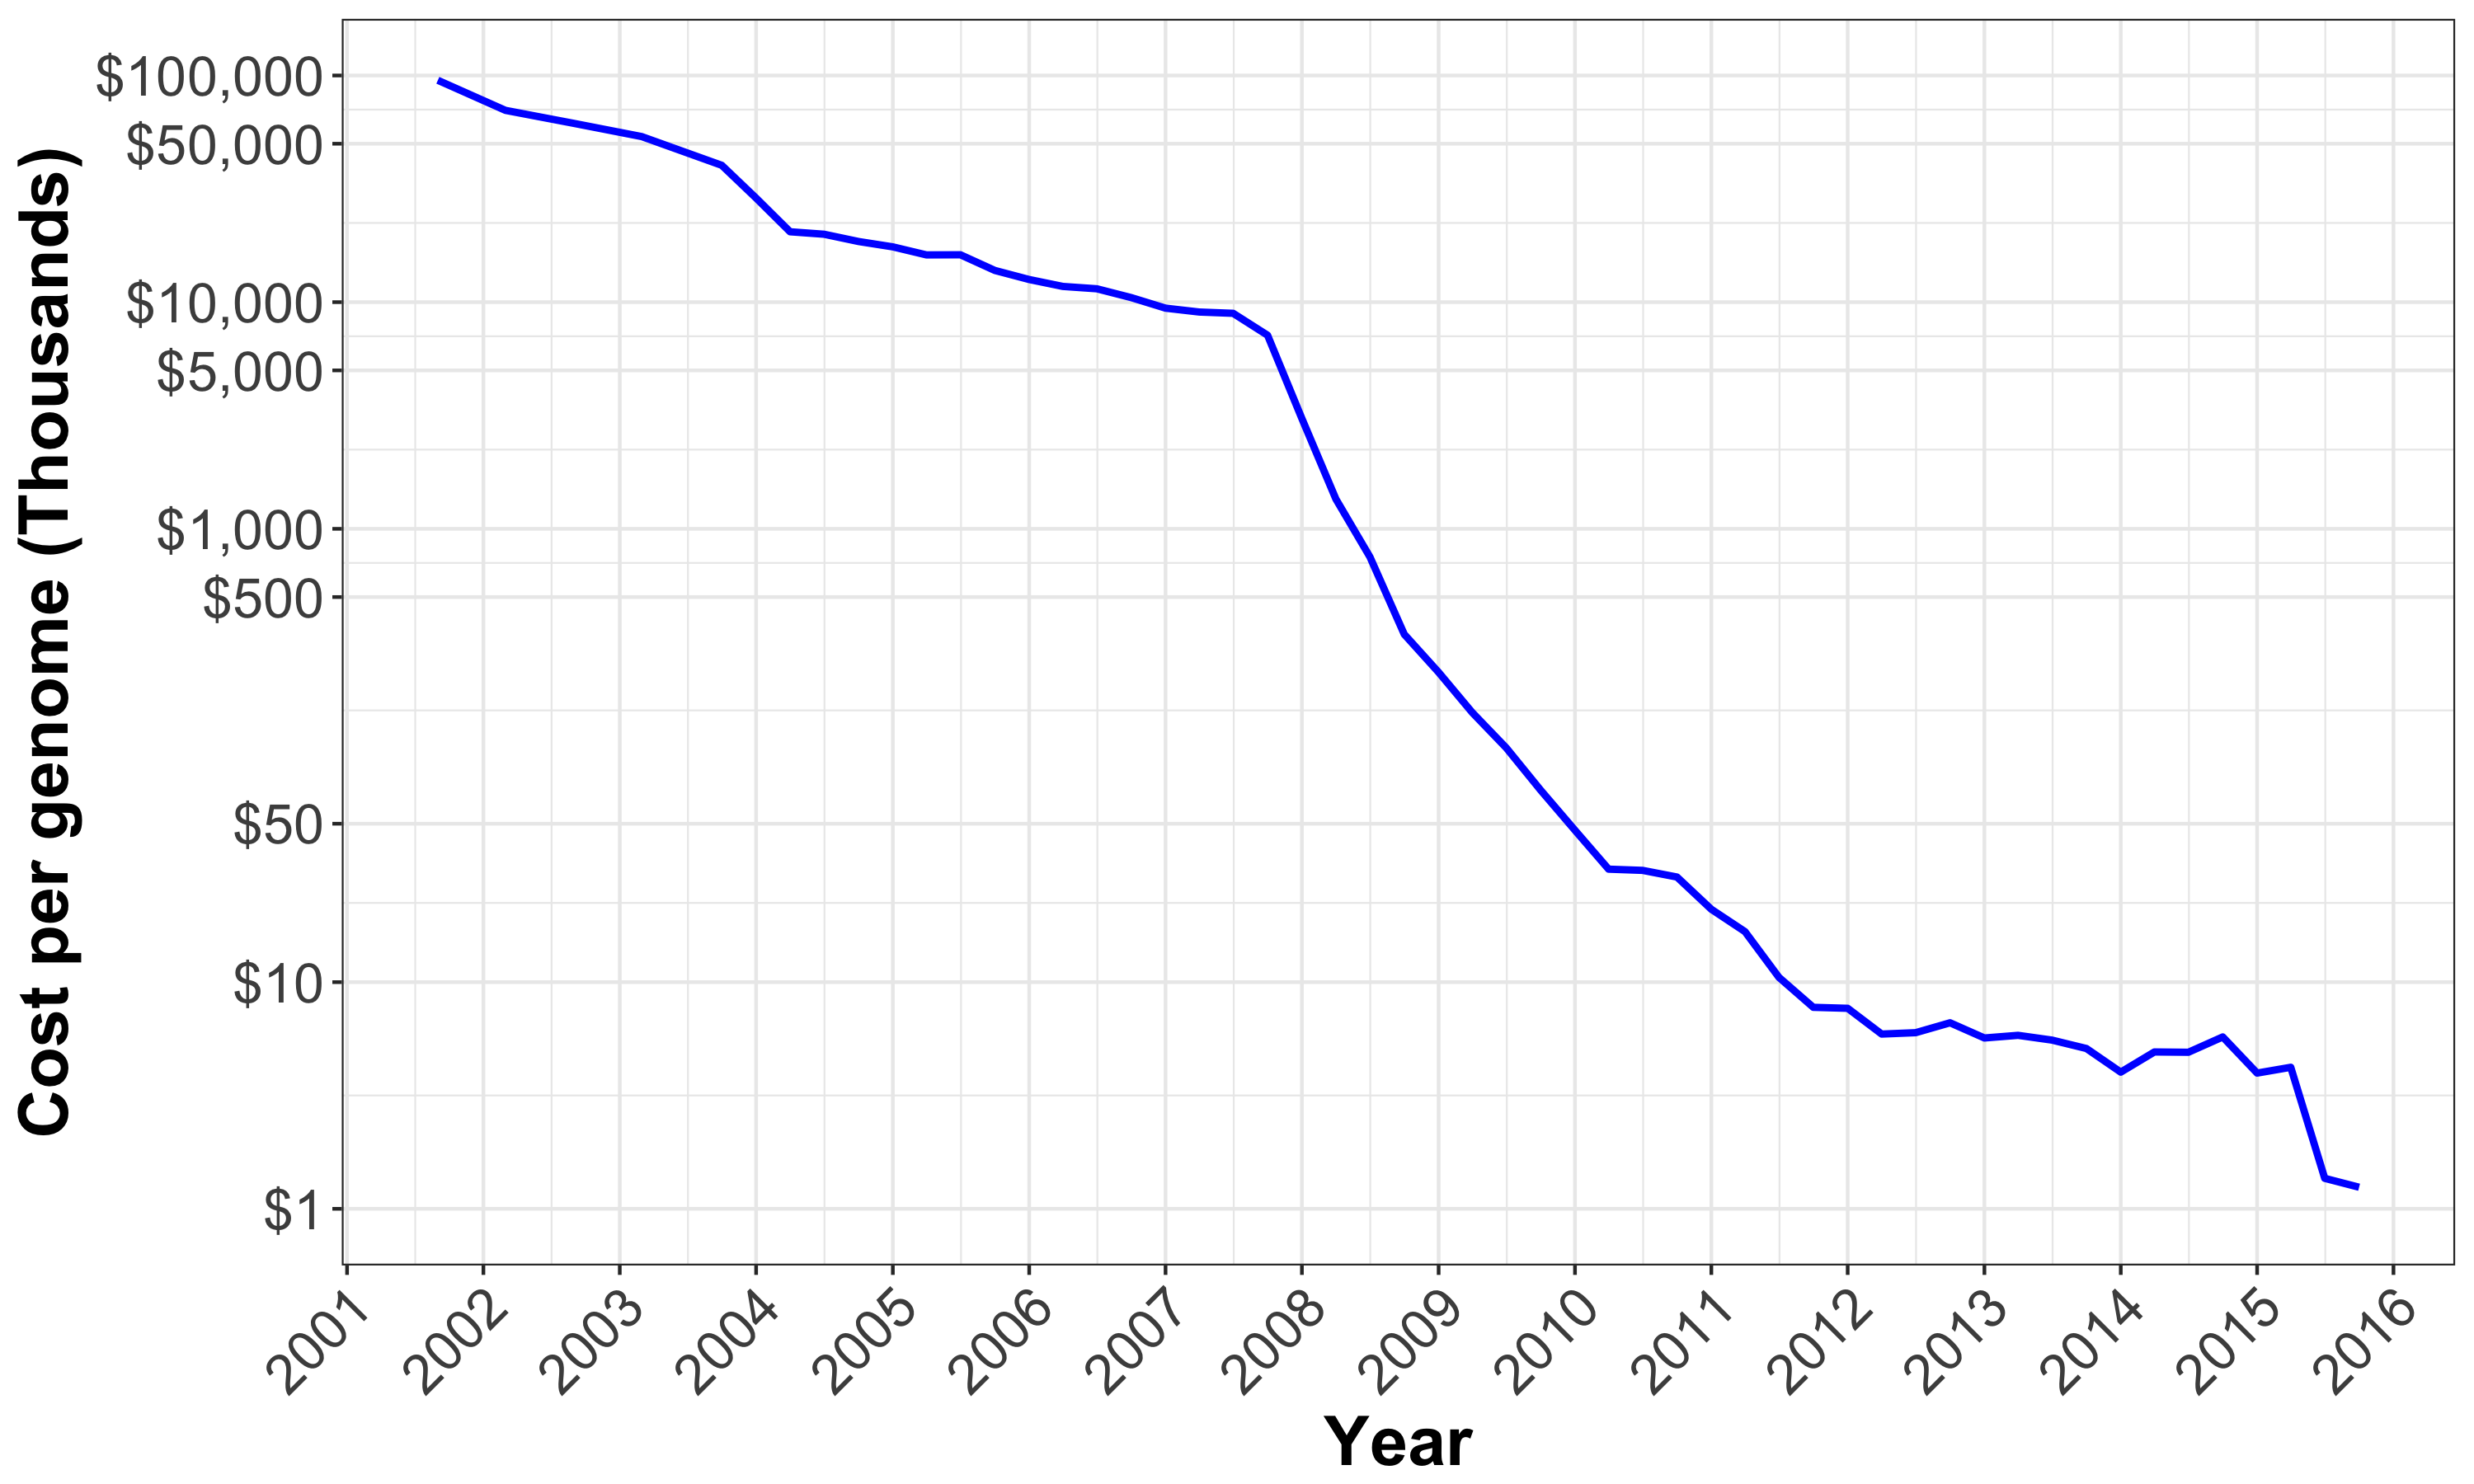
\includegraphics[scale=0.14]{cost_per_genome.png}
	\caption[Sequencing cost per human-sized genome between 2001 and 2015.]{Sequencing cost per human-sized genome between 2001 and 2015. Data by courtesy of the National Human Genome Research Institute (\acs{NHGRI}) \cite{Wetterstrand2016}.}
	\label{fig:cost_per_genome}
\end{figure}

%%%%%%%%%%%%%%%%%%%%%%%%%%%%%%%%%%%%%%%%%%%%%%%%%%%%%%%%%%%%%%%%%%%%%
%%%%%%%%%%%%%%%%%%%%%%%%%%%%%%%%%%%%%%%%%%%%%%%%%%%%%%%%%%%%%%%%%%%%%

%%%%%%%%%%%%%%%%%%%%%%%%%%%%%%%%%%%%%%%%%%%%%%%%%%%%%%%%%%%%%%%%%%%%%%
\newpage
\section{Overview of next-generation sequencing technologies}
\label{sec:Overviewofnext-generationsequencingtechnologies}

The Human Genome Project (\acs{HGP}) was completed in 2003, approximately 13 years after its launch date, producing the first human reference genome at an estimated expense of US\$2.7 billion \cite{NationalHumanGenomeResearchInstitute2010}. While the HGP provided a wealth of information, which led to major breakthroughs in the field of genomics, the completion time and cost of the project were apparent rate limiting steps. The need for more time- and cost-efficient DNA sequencing methods stimulated the development of NGS technologies. NGS is a general term that describes various high-throughout DNA sequencing technologies that can vary based on read length, chemistry, and detection methods (\autoref{tbl:ngs_platform_types}). These differences give rise to the strengths and weaknesses of each NGS platform. Recognition of these system specifications are essential for users to capitalize on the strengths and compensate for the limitations of the different NGS technologies.

In general, the sequencing process of most NGS platforms can be summarized into three steps. The first step involves nucleotide addition, which can be accomplished by DNA polymerase reaction or ligation (sequencing by synthesis \textit{vs.} sequencing by ligation). This is followed by a detection step to identify the nucleotide species that was incorporated on single molecule or clonally amplified DNA templates. Nucleotide detection can be performed using optical or non-optical sensing. Illumina and Pacific Biosciences (PacBio) platforms use optical sensing to detect fluorescence for base calling \cite{Bentley2008, Guo2008, Carneiro2012, English2012, Eid2009}, whereas the Ion Torrent platform uses non-optical sensing to detect change in pH to determine nucleotide identity \cite{Rothberg2011}. Lastly, a wash step re-initiates the cycle for the next base on the DNA templates by removing anchor-probe complexes or fluorophores and blocking groups. A key feature of NGS is its ability to simultaneously carry out this stepwise process for many millions of DNA templates; hence, NGS is also known as massively parallel sequencing. There are also NGS technologies that deviate from this sequencing cycle, such as the Oxford Nanopore Technologies (ONT) platform, which directly measures DNA sequence using current shifts produced as DNA translocates through nanopore sensors \cite{Wang2014}.

%%%%%%%%%%%%%%%%%%%%%%%%%%%%%%%%%%%%%%%%%%%%%%%%%%%%%%%%%%%%%%%%%%%%%
%%%%%%%%%%%%%%%%%%%%%%%%%%%%%%%%%%%%%%%%%%%%%%%%%%%%%%%%%%%%%%%%%%%%%

\newpage
\begin{landscape}

\begin{longtable}{p{0.2\linewidth}|p{0.1\linewidth}p{0.1\linewidth}p{0.2\linewidth}p{0.1\linewidth}p{0.25\linewidth}}
\caption[Different NGS platforms by read length, chemistry, and detection method.]{Different NGS platforms by read length, chemistry, and detection method. Adapted from a table created by \cite{Levy2016} under the \href{https://creativecommons.org/licenses/by/4.0/}{Creative Commons Attribution 4.0 International License}.}
\label{tbl:ngs_platform_types}
    \\
    \hline
    Platform & Read length\textsuperscript{$\dagger$} & Amplification & Chemistry & Detection & Website
		\\
    \hline
		Complete Genomics & Short & Clonal & Sequencing by ligation & Optical & \href{http://www.completegenomics.com/}{http://www.completegenomics.com/}
		\\
		Illumina & Short & Clonal & Sequencing by synthesis & Optical & \href{http://www.illumina.com}{http://www.illumina.com}
		\\
		Ion Torrent & Short & Clonal & Sequencing by synthesis & Solid state & \href{http://www.thermofisher.com/ca/en/home/brands/ion-torrent.html}{http://www.thermofisher.com/ca/en/\hspace{3pt}home/brands/ion-torrent.html}
		\\
		Oxford Nanopore & Long & Single molecule & Nanopore & Nanopore & \href{https://nanoporetech.com/}{https://nanoporetech.com/}
		\\
		Pacific Biosciences & Long & Single molecule & Sequencing by synthesis & Optical & \href{http://www.pacb.com/}{http://www.pacb.com/}
		\\
		Roche 454 & Short & Clonal & Sequencing by synthesis & Optical & \href{http://www.454.com}{http://www.454.com}
		\\
		\hbox{SoLiD, ThermoFisher} \mbox{Applied} Biosystems & Short & Clonal & Sequencing by ligation & Optical & \href{http://www.thermofisher.com/ca/en/home/brands/applied-biosystems.html}{http://www.thermofisher.com/ca/en/\hspace{3pt}home/brands/applied-biosystems.html}
		\\
		\hline
\end{longtable}
\noindent\textsuperscript{$\dagger$}Short-read platforms range from 35 bp to 700 bp, whereas long-read platforms range from 8 Kbp to 200 Kbp \cite{Goodwin2016}.
\end{landscape}

%%%%%%%%%%%%%%%%%%%%%%%%%%%%%%%%%%%%%%%%%%%%%%%%%%%%%%%%%%%%%%%%%%%%%
%%%%%%%%%%%%%%%%%%%%%%%%%%%%%%%%%%%%%%%%%%%%%%%%%%%%%%%%%%%%%%%%%%%%%

\subsection{Illumina sequencing}

At present, the most widely used NGS technology is the Illumina short-read platform as evident by its prevalence in the literature and the Sequence Read Archive (\acs{SRA}). In 2011, 84\% of sequence reads in the SRA were generated by Illumina sequencing \cite{Kodama2012}. The Illumina platform uses a sequencing-by-synthesis approach with reversible dye terminators, which enable base calling through detection of fluorescent signals while blocking the ribose 3'-OH group to prevent addition of the next nucleotide by DNA polymerase \cite{Bentley2008, Guo2008}. Briefly, an Illumina NGS workflow begins by ligating adapters to the ends of fragmented DNA, followed by hybridizing these templates to complementary adapter sequences on flow cell surfaces. Bridge amplification is then performed to generate clusters of clonally amplified DNA templates. DNA sequencing starts by annealing primers complementary to adapter sequences, which enable DNA polymerase to carry out the elongation process. All four reversible dye terminator-bound deoxyribonucleotides (\acs{dNTP}s) are simultaneously added during each cycle and are distinguishable by unique fluorophore-labelling. The dNTPs are also terminally blocked, allowing the incorporation of only one dNTP molecule per cycle. Subsequent to dNTPs addition, unbound dNTPs are washed away. The flow cells are then imaged using laser channels and fluorescence corresponding to the incorporated dNTP is emitted at each cluster. Finally, a new cycle is initiated by cleaving the fluorophores and unblocking the 3'-OH groups (\autoref{fig:illumina}) \cite{Mardis2013, Goodwin2016, Levy2016, Mardis2017}.

%%%%%%%%%%%%%%%%%%%%%%%%%%%%%%%%%%%%%%%%%%%%%%%%%%%%%%%%%%%%%%%%%%%%%
%%%%%%%%%%%%%%%%%%%%%%%%%%%%%%%%%%%%%%%%%%%%%%%%%%%%%%%%%%%%%%%%%%%%%

\newpage
\begin{landscape}

\begin{figure}[H]
	\centering
	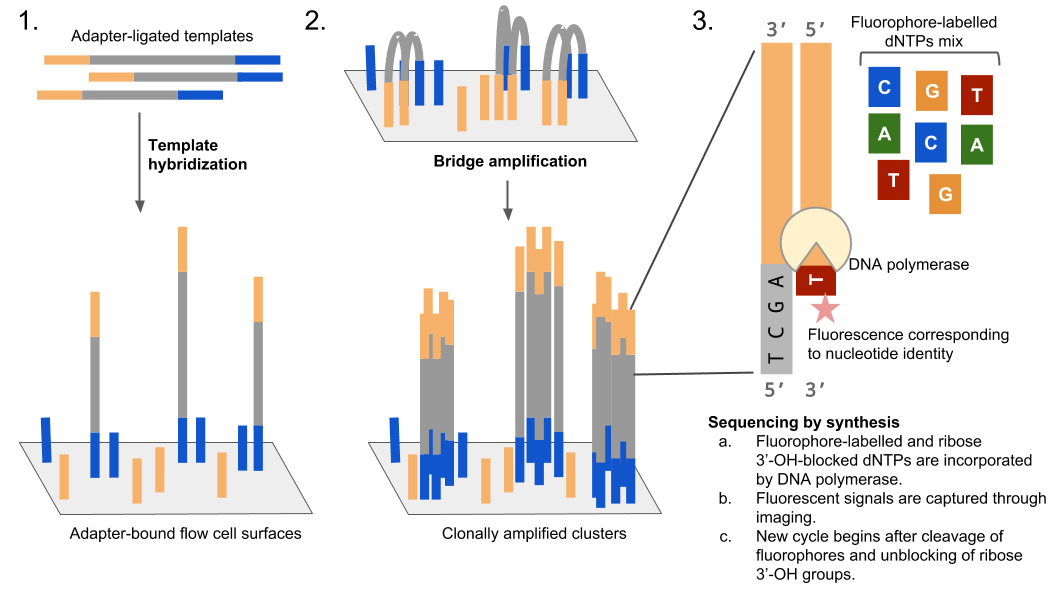
\includegraphics[scale=0.6]{illumina.png}
	\caption[Workflow for Illumina sequencing.]{Workflow for Illumina sequencing. (1) Hybridization of adapter-ligated templates to flow cell surfaces. (2) Bridge amplification to generate clonally amplified clusters. (3) Sequencing by synthesis.}
	\label{fig:illumina}
\end{figure}

\end{landscape}

%%%%%%%%%%%%%%%%%%%%%%%%%%%%%%%%%%%%%%%%%%%%%%%%%%%%%%%%%%%%%%%%%%%%%
%%%%%%%%%%%%%%%%%%%%%%%%%%%%%%%%%%%%%%%%%%%%%%%%%%%%%%%%%%%%%%%%%%%%%

\subsection{Clinical applications of NGS}

The emergence of NGS has revolutionized biological inquiry, particularly in cancer genomics research. Collaborative efforts such as The Cancer Genome Atlas (\acs{TCGA}) and the International Cancer Genome Consortium (\acs{ICGC}) have leveraged NGS technologies to characterize genomic landscapes of different subtypes of tumours \cite{Robertson2017, Raphael2017, Ally2017, Nik-Zainal2016, Tirode2014}. This has resulted in the identification of novel driver mutations, thereby enhancing knowledge of tumour biology and treatment strategies. The ability to sequence multiple genes and samples in parallel with less DNA and in a cost- and time-effective manner, also makes NGS an attractive clinical tool to complement precision medicine initiatives. These advantages demonstrate that the viability and efficiency of NGS are superior to traditional Sanger sequencing, which is typically limited to sequencing a specific gene region of a given sample per run. Currently, tumour sequencing assays ranging from targeted gene panels up to genome-scale profiling have been employed in clinical oncology to guide diagnosis, prognosis, and therapeutic decision-making (\autoref{fig:clinical_app_ngs}).

%%%%%%%%%%%%%%%%%%%%%%%%%%%%%%%%%%%%%%%%%%%%%%%%%%%%%%%%%%%%%%%%%%%%%
%%%%%%%%%%%%%%%%%%%%%%%%%%%%%%%%%%%%%%%%%%%%%%%%%%%%%%%%%%%%%%%%%%%%%

\begin{figure}[H]
	\centering
	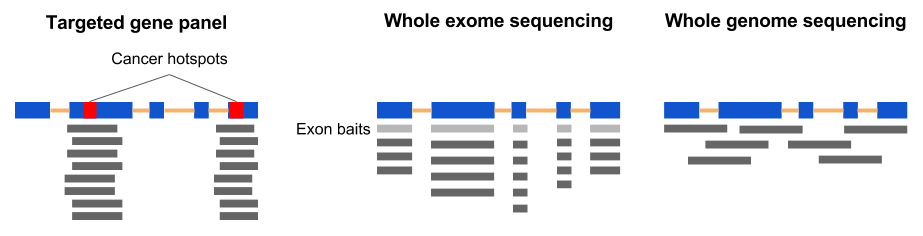
\includegraphics[scale=0.45]{clinical_app_ngs.png}
	\caption{Comparison of testing content across targeted gene panels, whole exome sequencing, and whole genome sequencing.}
	\label{fig:clinical_app_ngs}
\end{figure}

%%%%%%%%%%%%%%%%%%%%%%%%%%%%%%%%%%%%%%%%%%%%%%%%%%%%%%%%%%%%%%%%%%%%%
%%%%%%%%%%%%%%%%%%%%%%%%%%%%%%%%%%%%%%%%%%%%%%%%%%%%%%%%%%%%%%%%%%%%%

\vspace{5mm}
\noindent\textit{Targeted gene panels}

Several considerations must be made when developing clinical-grade tumour genomic tests, including turnaround time, testing cost per patient, and depth of sequencing coverage. For these reasons, many clinical laboratories have resorted to targeted gene panels, which focus on mutational hotspots, actionable genes, or genomic regions of known clinical relevance. Furthermore, despite the growing catalog of tumour genetic variants contributed by large consortium projects, the impact of the majority of variants on cancer development remains unknown \cite{Sukhai2016, Strom2016, Richards2015}. Genomic information of unknown significance not only pose limitations in clinical translation, but also challenges in communicating such results to patients \cite{Culver2013, Strom2016, Richards2015, Scherr2015}. Hence, targeted gene panels are more practical for prospective clinical use at the present time than whole exome and genome approaches.

Strategies to interrogate genomic regions of interest in targeted NGS assays include amplicon-based and capture-based methods (\autoref{fig:targeted_ngs}). Amplicon-based method enriches target regions using PCR amplification prior to NGS. PCR can be performed in uniplex, in which a single primer pair is used to generate amplicons within one reaction, or in multiplex, in which multiple primer pairs are used to generate amplicons in a single reaction. Conventional multiplex PCR faces challenges such as interactions between primers and competition for reagents, which could lead to amplification failures. These limitations of conventional multiplex PCR can be circumvented by the microdroplet-based PCR platform developed by RainDance Technologies. In microdroplet-based PCR enrichment, droplets containing a single primer pair are merged with droplets of fragmented genomic DNA. PCR enrichment is then performed for a library of droplets, which simultaneously amplifies several target regions in a single reaction. Within each PCR droplet, amplicon generation is confined to a single primer pair and other reagents. This eliminates interaction between primer pairs and competition for reagents, thereby enhancing amplification uniformity \cite{Mamanova2010}.

The amplicon-based approach typically requires lower amount of DNA input and offers quick turnaround relative to hybridization capture methods \cite{Chang2013, Gagan2015}. However, \acs{PCR} amplification can distort detection of copy number variation (\acs{CNV}), although bioinformatics tools, such as ONCOCNV \cite{Boeva2014}, have been developed to perform copy number analysis using amplicon sequencing data. Moreover, amplicon sequencing is prone to enrichment bias, especially in samples with low amounts of DNA templates. For example, Wong et al. \cite{Wong2014} reported higher prevalence of formalin-induced sequence artifacts in samples with lower amounts of amplifiable templates. Clinical specimens with low template copies tend to have reduced amplicon enrichment and higher probability of amplifying DNA templates with sequence artifacts \cite{Wong2014}. Another limitation of amplicon sequencing is its inability to detect novel gene fusions because PCR primer pairs would fail to amplify the translocated DNA \cite{Simon2013, Gagan2015}.

Hybridization capture methods involve the use of complementary oligonucleotide probes to bind targeted regions. There are two methods for target capture, namely array-based and in-solution capture (\autoref{fig:targeted_ngs}B). In array-based capture, complementary oligonucleotide probes of targeted regions are fixed on microarrays. Fragmented genomic DNA is hybridized to the probes on the microarray and subjected to NGS after unbound DNA is washed away. In the in-solution capture approach, the target-specific probes are biotinylated. The pool of probes is mixed with fragmented genomic DNA and hybridization occurs ``in solution." Hybridized DNA is pulled down using streptavidin-labelled magnetic beads and then subjected to NGS \cite{Simon2013, Gagan2015}. The in-solution capture method is typically preferred over array-based capture because it omits the necessity for expensive instrument to process microarrays, and it requires lower quantity of DNA as starting material \cite{Bodi2013, Cui2013}. In contrast to the amplicon-based method, hybridization capture approaches can detect gene fusions, as well as yield more reliable inference of CNVs \cite{Simon2013, Gagan2015}.

%%%%%%%%%%%%%%%%%%%%%%%%%%%%%%%%%%%%%%%%%%%%%%%%%%%%%%%%%%%%%%%%%%%%%
%%%%%%%%%%%%%%%%%%%%%%%%%%%%%%%%%%%%%%%%%%%%%%%%%%%%%%%%%%%%%%%%%%%%%

\begin{figure}[H]
	\centering
	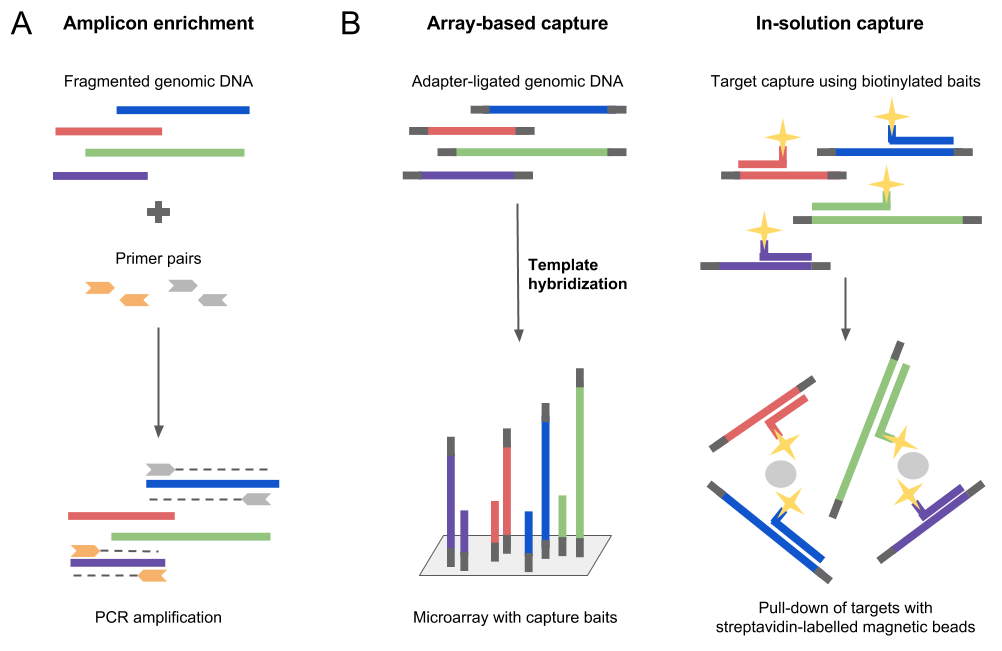
\includegraphics[scale=0.45]{targeted_ngs.png}
	\caption[Different approaches in target enrichment.]{Different approaches in target enrichment. (A) Amplicon-based enrichment. (B) Capture-based enrichment, which can be categorized as array-based and in-solution capturing.}
	\label{fig:targeted_ngs}
\end{figure}

%%%%%%%%%%%%%%%%%%%%%%%%%%%%%%%%%%%%%%%%%%%%%%%%%%%%%%%%%%%%%%%%%%%%%
%%%%%%%%%%%%%%%%%%%%%%%%%%%%%%%%%%%%%%%%%%%%%%%%%%%%%%%%%%%%%%%%%%%%%

\newpage
\vspace{5mm}
\noindent\textit{Whole exome sequencing}

Whole exome sequencing (\acs{WES}) interrogates all protein-coding regions, which constitute approximately 1\% of the genome \cite{Simon2013, Rabbani2014}. Target capture methods are commonly used to enrich coding sequences before massively parallel sequencing. To date, it is estimated that 85\% of pathogenic variants are present within exons \cite{Rabbani2014}. Therefore, WES assays have the potential to facilitate prospective medical decision-making, as well as contribute to retrospective studies to uncover the functional and clinical impacts of newly discovered genetic alterations in tumours.

There are several disadvantages associated with WES assays. This includes the inability to detect mutations in non-coding regions and structural variants, which can promote cancer formation. WES assays also tend to achieve lower depth of coverage compared to targeted gene panels, increasing the rates of false positives. Because of the increased testing content, analytical validation of WES assays is more challenging and time-consuming. Nevertheless, whole exome testing has already been offered by a few academic centres such as Broad Institute of \acs{MIT} and Harvard, Baylor College of Medicine, and Washington University in St. Louis, to assist in precision cancer medicine \cite{Simon2013, Rabbani2014}.

\vspace{5mm}
\noindent\textit{Whole genome sequencing}

Whole genome sequencing (\acs{WGS}) scans the entire genome, including coding and non-coding genomic regions. Similar to WES, WGS faces drawbacks in terms of depth of coverage and difficulty in ensuring analytic validity \cite{Simon2013}. Although the Illumina HiSeq X Ten System has made it possible to sequence an entire genome at 30x coverage under US\$1000 \cite{Dong2015}, application of WGS in routine clinical testing is still challenging due to limitations in variant interpretation. As a result of limited clinically annotated genetic variants, WGS is expected to yield a high burden of variants of unknown significance, which are problematic in clinical practice \cite{Rehm2013, Simon2013}. Despite these constraints, Laskin et al. \cite{Laskin2015} reported that the Personalized OncoGenomics (POG) study, which integrates whole genome analysis in making therapeutic decision, can benefit patients with advanced cancers by matching them with targeted agents that are approved or currently in clinical trials. Thus, while there are challenges that need to be overcome to implement WGS as standard of care, WGS has proven its utility in conducting additional search for actionable mutations that are undetected by less comprehensive sequencing strategies. In particular, follow-up testing with WGS can broaden the treatment options for patients with incurable cancers.

%%%%%%%%%%%%%%%%%%%%%%%%%%%%%%%%%%%%%%%%%%%%%%%%%%%%%%%%%%%%%%%%%%%%%%
\section{Variant analysis pipeline}
\label{sec:Variantanalysispipeline}

The increase in affordability of NGS technologies has led to a marked surge in data production. For instance, the Illumina HiSeq 2500 platform is capable of sequencing 150--180 whole exomes from human samples at 50x coverage, generating approximately 1TB of raw data in a single run \cite{Dong2015}. Processing these enormous data sets and extracting useful results for research and clinical purposes rely heavily on bioinformatics algorithms and tools. A general workflow for variant analysis in medical genomics consists of four stages: (1) quality control and pre-processing of raw sequencing reads, (2) read alignment to the reference genome and post-alignment processing, (3) variant calling, and (4) variant annotation and interpretation.

\subsection{Quality control and pre-processing of raw sequencing reads}

Base-calling algorithms convert signals, such as fluorescence, light intensity, or electrical current, captured by NGS instruments to DNA sequences. For each base identified, a measure of uncertainty, known as base quality (\acs{BAQ}) score, is derived by taking into account background noise. BAQ scores are commonly reported in Phred scale, given by the equation below. $$BAQ\textsubscript{Phred} = -10log\textsubscript{10}P(error)$$ Hence, 1$/$1000 probability of base error would correspond to a Phred-scaled BAQ score of 30 \cite{Nielsen2011a, Ledergerber2011}.

The raw output of NGS instruments, which contains information from base calling, are stored in FASTQ and FASTA text-based formats. FASTQ files contain DNA sequences with sequence names and Phred-scaled BAQ scores, whereas FASTA files only contain DNA sequences with sequence names (\autoref{fig:fasta_fastq}) \cite{Bao2014, Mielczarek2016}. Quality of raw NGS data can be evaluated using bioinformatics tools such as FastQC, which generates a diagnostic report consisting of various quality control parameters. These include sequence length distribution, GC content distribution, degree of sequence duplication, presence of overrepresented and adapter sequences, and average Phred-scaled BAQ scores at each base across reads \cite{Andrews2017}.

Quality control results are used to assist in pre-processing of raw NGS data before further analysis takes place. For example, NGS libraries with poor quality bases near the 3' ends of reads may require read trimming before alignment. Removal of adapters is also typically performed in the pre-processing step \cite{Bao2014}. Computational tools that are commonly used to accomplish these tasks include Trimmomatic \cite{Bolger2014} and Cutadapt \cite{Marcel2011}. Moreover, assessment of quality control metrics also enables the recognition of poor quality NGS libraries and those that are potentially contaminated. Flagging of these libraries would allow downstream analyses and result interpretation to be performed with caution.

%%%%%%%%%%%%%%%%%%%%%%%%%%%%%%%%%%%%%%%%%%%%%%%%%%%%%%%%%%%%%%%%%%%%%
%%%%%%%%%%%%%%%%%%%%%%%%%%%%%%%%%%%%%%%%%%%%%%%%%%%%%%%%%%%%%%%%%%%%%

\begin{figure}[H]
	\centering
	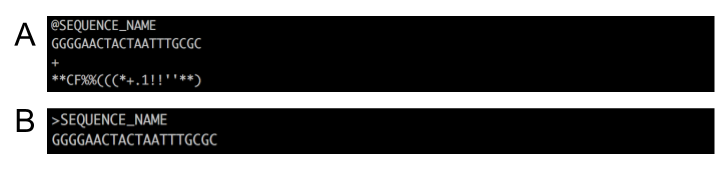
\includegraphics[scale=0.6]{fasta_fastq.png}
	\caption[File formats of raw output from NGS instruments.]{File formats of raw output from NGS instruments. (A) FASTQ format. Sequence name starting with $@$ is presented in line 1, followed by read sequence in line 2. Line 3 begins with + and may be followed by the sequence name again, and line 4 consists of quality scores corresponding to bases in line 2. Quality scores are represented as  \acs{ASCII} characters. (B) FASTA format. Line 1 contains sequence name, which starts with $>$, whereas line 2 contains the read sequence.}
	\label{fig:fasta_fastq}
\end{figure}

%%%%%%%%%%%%%%%%%%%%%%%%%%%%%%%%%%%%%%%%%%%%%%%%%%%%%%%%%%%%%%%%%%%%%
%%%%%%%%%%%%%%%%%%%%%%%%%%%%%%%%%%%%%%%%%%%%%%%%%%%%%%%%%%%%%%%%%%%%%

\subsection{Read alignment and post-alignment processing}

Next, pre-processed reads are aligned to the reference genome. Alignment algorithms essentially match read sequences to sequences in the reference genome, while accounting for sequencing errors and true genomic alterations \cite{Bao2014, Nielsen2011a, Mielczarek2016, Li2010}. Because of the large data output produced by NGS, alignment algorithms must also be time- and memory-efficient.

Widely-used alignment softwares implement either the Burrows-Wheeler transform (\acs{BWT}) compression algorithm or hash table indexing \cite{Bao2014, Nielsen2011a, Pabinger2014, Li2010}. Popular BWT-based aligners include BWA \cite{Li2009, Li2010a, Li2012} and Bowtie2 \cite{Langmead2013}, which are well-known for reduced runtimes and memory requirements. Conversely, algorithms based on hash tables such as Novoalign (http://novocraft.com), SHRiMP2 \cite{David2011}, and Stampy \cite{Lunter2011} have longer computational times but tend to yield more accurate alignments \cite{Bao2014, Nielsen2011a, Li2010}. The standard formats for storing aligned read data are the Sequence Alignment$/$Map (\acs{SAM}) text-based format and its compressed binary version, the Binary Alignment$/$Map (\acs{BAM}) format \cite{Li2009b}.

Several post-alignment steps are performed such as removal of read duplicates, which could be introduced by PCR bias. Local realignment is also often performed at genomic regions surrounding insertions-deletions (indels) to reduce errors caused by inaccurate alignments. As raw BAQ scores might be erroneously assigned, recalibration of BAQ scores is sometimes recommended prior to variant calling. Quality scores are adjusted by accounting for differences in quality between machine cycles and neighbouring dinucleotides \cite{Bao2014, Mielczarek2016, Nielsen2011a, Oliver2015}.

\subsection{Variant calling}

Variant calling identifies genomic differences between aligned read sequences and the reference genome. When matched normal samples are sequenced, some variant callers are able to detect germline, somatic, and loss of heterozygosity (\acs{LOH}) events through paired analysis of tumour and matched normal samples \cite{Koboldt2013}. Variant callers can be categorized as heuristic or probabilistic \cite{Mielczarek2016, Pabinger2014, Bao2014}. The standard output of variant callers for storing sequence variant data is the text-based Variant Call Format (\acs{VCF}) (\autoref{fig:vcf}) \cite{Danecek2011}.

VarScan2 is a variant caller that uses heuristic factors like cut-offs for coverage depth, BAQ score, and variant allele frequency (\acs{VAF}), as well as the one-sided Fisher's exact test (\acs{FET}) on mapped read counts to identify variants \cite{Bao2014, Pabinger2014, Mielczarek2016, Koboldt2013, Koboldt2012}. In single sample analysis (sample \textit{vs.} reference genome), a variant is detected through applying the one-sided FET to compare reference- and variant-supporting read counts to an expected read distribution that reflects sequencing error rate at a reference site \cite{Koboldt2013, Koboldt2012}. For example, the expected read distribution would comprise 1998 reference-supporting reads and 2 variant-supporting reads, which are reads with errors, for a reference site with 2000x coverage depth if the sequencing error rate is 0.1\%.

Variant callers that are based on probabilistic methods employ Bayes' theorem to measure posterior probabilities of all possible genotypes at a loci. These posterior probabilities are then used to infer genotype. Probabilistic methods also take into account prior information such as population allele frequencies, which can be obtained from the Single Nucleotide Polymorphism Database (dbSNP) or through multi-sample variant calling, and patterns of linkage disequilibrium, as well as genotype likelihood, which can be computed using BAQ scores \cite{Mielczarek2016, Nielsen2011a}. Examples of variant callers that implement probabilistic approaches include GATK \cite{Schmidt2009}, MuTect \cite{Cibulskis2013}, and Strelka \cite{Saunders2012}.

%%%%%%%%%%%%%%%%%%%%%%%%%%%%%%%%%%%%%%%%%%%%%%%%%%%%%%%%%%%%%%%%%%%%%
%%%%%%%%%%%%%%%%%%%%%%%%%%%%%%%%%%%%%%%%%%%%%%%%%%%%%%%%%%%%%%%%%%%%%

\begin{figure}[H]
	\centering
	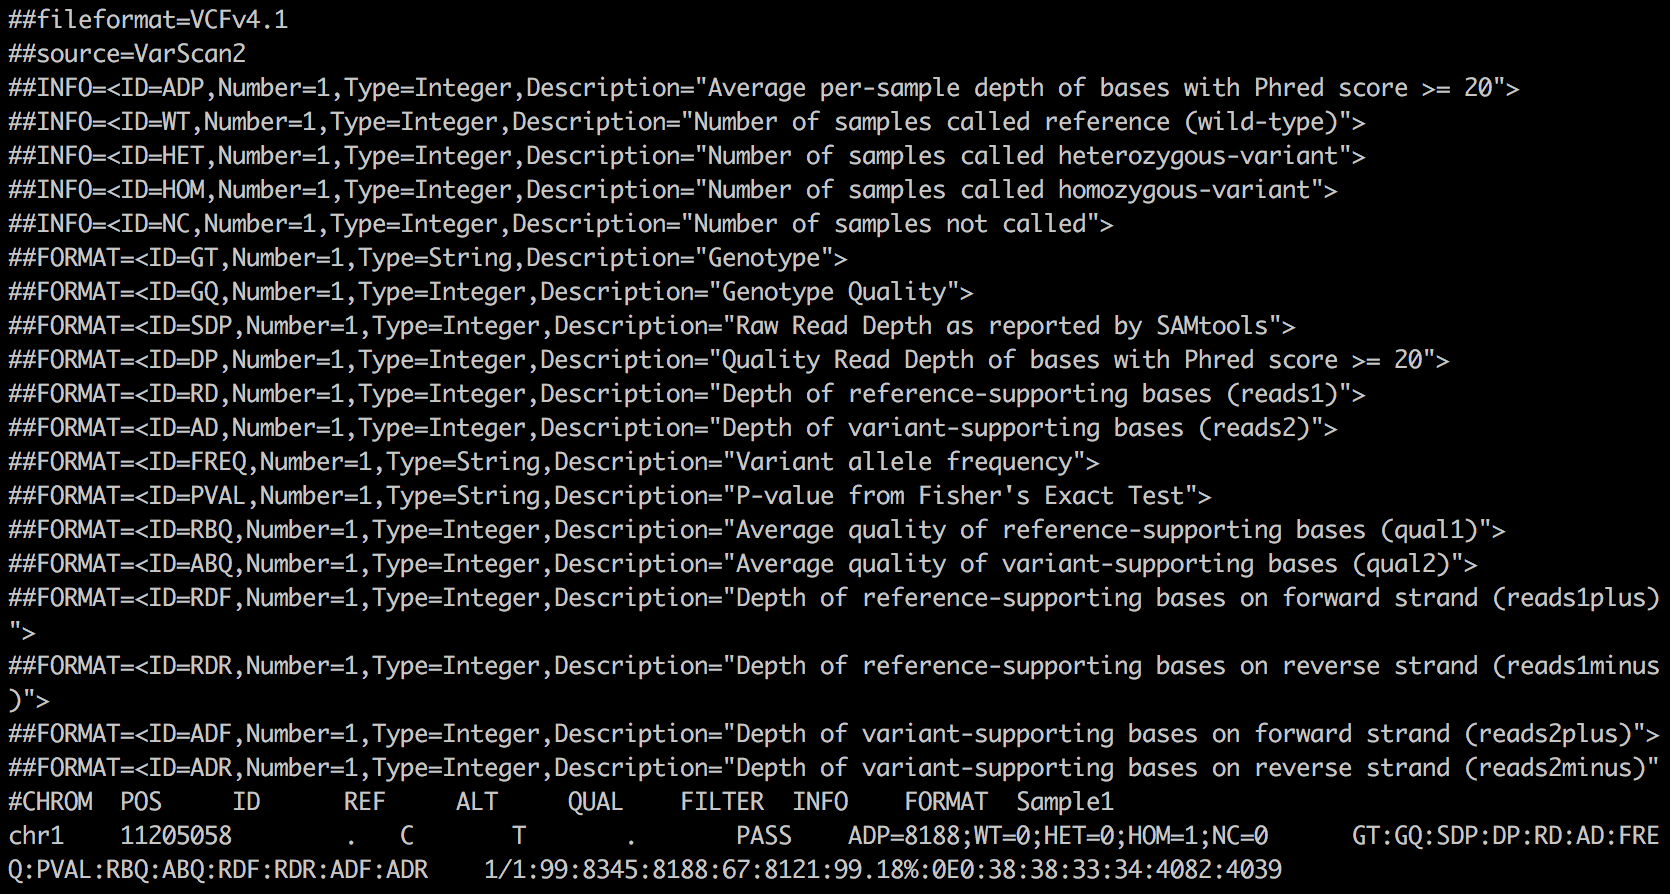
\includegraphics[scale=0.5]{vcf.png}
	\caption[VCF format for storing sequence variation data.]{VCF format for storing sequence variation data. The VCF header, which begins with \#\#, contains information describing the data in the file. The line starting with \# displays the column names and indicates the beginning of the body of the VCF file. Data columns must include eight mandatory fields: chromosome (CHROM), 1-based genomic position of the variant (POS), variant identifier (ID), reference base (REF), alternate base (ALT), quality score (QUAL), indicator whether the variant passed the specified filtering criteria (FILTER), variant annotations separated by semicolon (INFO). The FORMAT field contains colon-separated descriptors of the values in the genotype column, which is named after the sample(s) reported in the VCF file \cite{Danecek2011}.}
	\label{fig:vcf}
\end{figure}

%%%%%%%%%%%%%%%%%%%%%%%%%%%%%%%%%%%%%%%%%%%%%%%%%%%%%%%%%%%%%%%%%%%%%
%%%%%%%%%%%%%%%%%%%%%%%%%%%%%%%%%%%%%%%%%%%%%%%%%%%%%%%%%%%%%%%%%%%%%

\subsection{Variant annotation and interpretation}

Subsequent to variant calling, variant annotation is performed by adding structural and functional information. Structural annotation provides information on the genomic location of the variant (e.g. intronic, intergenic, 5'UTR, 3'UTR, \textit{etc.}), the impact of the variant on the gene transcript (e.g. missense, non-synonymous, synonymous, frameshift, \textit{etc.}), and changes in codon and amino acid \cite{Moorthie2013, Bao2014, Oliver2015}. These information are typically reported in the Human Genome Variation Society (HGVS) nomenclature to ensure a consistent format in describing sequence variants \cite{DenDunnen2016}.

Functional annotation, on the other hand, provides information on the effect of genomic variants on protein function. Pathogenicity of a variant cannot be exclusively presumed based on the predicted variant effect. For example, not all truncating, missense, and frameshift variants lead to deleterious effects. Conversely, not all synonymous variants are benign. Thus, functional prediction algorithms compute functional inference by incorporating additional data such as sequence homology, 3D protein structure, genomic context, protein interaction network, and evolutionary conservation \cite{Quintans2014, Oliver2015}. Examples of functional prediction tools include PolyPhen-2 \cite{Adzhubei2010}, SIFT \cite{Ng2003}, MutPred \cite{Li2009a}, Condel \cite{Gonzalez-Perez2011}, and PhD-SNP \cite{Capriotti2006}.

Population allele frequencies are also taken into account when interpreting variants \cite{Oliver2015, Bao2014, Moorthie2013}. For instance, a common variant (minor allele frequency $>$1\%) is unlikely to be involved in cancer predisposition \cite{Baynes2007, Baker2006}. Population allele frequencies can be obtained by annotating variants with the dbSNP and Exome Aggregation Consortium (\acs{ExAC}) database. Furthermore, variant databases such as ClinVar and Catalogue of Somatic Mutations in Cancer (\acs{COSMIC}) are also useful resources that provide information on clinical significance of variants and presence of variants in cancers \cite{Oliver2015, Moorthie2013}.

The original output of variants is then filtered and prioritized based on the different types of annotations, as well as clinical and biological relevance, generating a list of candidate variants \cite{Moorthie2013, Oliver2015}. These variants are typically visualized using a genomic browser like the Intergrative Genomics Viewer (\acs{IGV}) for quality control purposes \cite{Oliver2015, Pabinger2014}. Finally, a report is produced and reviewed by a board certified medical pathologist or clinical molecular geneticist for approval \cite{Moorthie2013, Strom2016}.

%%%%%%%%%%%%%%%%%%%%%%%%%%%%%%%%%%%%%%%%%%%%%%%%%%%%%%%%%%%%%%%%%%%%%%
\section{ACCE model process for evaluating genetic tests}
\label{sec:ACCEmodelprocessforevaluatinggenetictests}

Development of a genetic test, including NGS-based genomic testing, for clinical use must be accompanied by an evaluation process to establish robustness and clinical benefits of the test. One approach to assess genetic tests is the \acs{ACCE} model process, which consists of four criteria that make up its acronym: \textbf{A}nalytical validity, \textbf{C}linical validity, \textbf{C}linical utility, and \textbf{E}thical, legal and social implications \cite{Sanderson2005, Zimmern2007}.

Analytic validation ensures that a clinical assay detects the genetic changes it is designed to identify with sufficient sensitivity and specificity \cite{Sanderson2005, Zimmern2007}. For example, analytic validity of a targeted NGS panel can be determined by running the panel on samples with known mutations that were previously identified using Sanger sequencing. Sensitivity and specificity of the targeted NGS panel can be measured using the results from Sanger sequencing as reference standards. Analytic validity also refers to quality assurance of a clinical assay. For instance, a targeted NGS panel must be capable of producing similar sequencing metrics (e.g. read depth and coverage uniformity) for samples with comparable DNA quantity and integrity.

Clinical validation determines whether results of the genetic test correspond to the clinical condition it is meant to detect \cite{Sanderson2005, Zimmern2007}. Example of a genetic test with high clinical validity is \acs{RET} mutational testing, which can identify individuals with multiple endocrine neoplasia type 2 (\acs{MEN2}) at a sensitivity of 95--98\%. MEN2 is a heritable disorder transmitted in an autosomal dominant pattern, resulting in increased susceptibility to tumours in endocrine tissues, especially medullary thyroid carcinoma \cite{Burke2014}. On the other hand, clinical utility of a genetic test is defined by its ability to enhance clinical outcome, such as survival and progression-free survival, after weighing in the risks, benefits, and economic impact of the test \cite{Sanderson2005, Zimmern2007}. The clinical utility of \acs{RET} mutational testing is demonstrated by its efficacy in identifying MEN2 susceptible children who would benefit from prophylactic surgery to remove all or parts of the thyroid gland. This results in reduced risk of developing thyroid cancers, thereby improving survival of these individuals \cite{Burke2014}.

Lastly, the ACCE model includes evaluation of ethical, legal and social implications of a genetic test. This component considers how the genetic test can lead to ramifications such as violation of privacy and confidentiality, stigmatization and discrimination based on genetic makeup (e.g. accessibility to insurance), and complications pertaining to consent for disclosure and ownership of the data. As well, this component of the framework ensures that safeguards, such as relevant policies and genetic counseling protocols, are implemented to prevent societal repercussions \cite{Sanderson2005, Zimmern2007}.

%%%%%%%%%%%%%%%%%%%%%%%%%%%%%%%%%%%%%%%%%%%%%%%%%%%%%%%%%%%%%%%%%%%%%
%%%%%%%%%%%%%%%%%%%%%%%%%%%%%%%%%%%%%%%%%%%%%%%%%%%%%%%%%%%%%%%%%%%%%

\begin{figure}[H]
	\centering
	\includegraphics[scale=0.6]{acce_wheel.png}
	\caption[Four main criteria of the ACCE model process for evaluating a genetic test: \textbf{A}nalytical validity, \textbf{C}linical validity, \textbf{C}linical utility, and \textbf{E}thical, legal and social implications.]{Four main criteria of the ACCE model process for evaluating a genetic test: \textbf{A}nalytical validity, \textbf{C}linical validity, \textbf{C}linical utility, and \textbf{E}thical, legal and social implications. Image by courtesy of Centers for Disease Control and Prevention (\acs{CDC}).}
	\label{fig:acce_wheel}
\end{figure}

%%%%%%%%%%%%%%%%%%%%%%%%%%%%%%%%%%%%%%%%%%%%%%%%%%%%%%%%%%%%%%%%%%%%%
%%%%%%%%%%%%%%%%%%%%%%%%%%%%%%%%%%%%%%%%%%%%%%%%%%%%%%%%%%%%%%%%%%%%%


%%%%%%%%%%%%%%%%%%%%%%%%%%%%%%%%%%%%%%%%%%%%%%%%%%%%%%%%%%%%%%%%%%%%%%
\section{Clinical implications of germline alterations in cancer}
\label{sec:Clinicalimplicationsofgermlinealterationsincancer}

Screening for somatic and germline alterations are essential in delivering precision medicine to cancer patients. Somatic mutations can influence disease management and treatment of cancer patients with targeted agents, whereas clinical implications of germline alterations extend beyond the patients, affecting their families as well. Germline variants in cancer predisposing genes (\acs{CPG}s) can predict the risk of disease onset, allowing for preventive measures to be administered \cite{Rahman2014}. Furthermore, germline variants in pharmacogenomic (\acs{PGx}) genes can predict response to chemotherapeutic drugs, including drug sensitivity and adverse drug reactions \cite{Panczyk2014, Mohelnikova-Duchonova2014}. Therefore, germline testing should be offered to ensure more precise cancer care if resources are available to analyze and interpret germline findings, and appropriate protocols are established to communicate results with patients and affected family members.

\subsection{Cancer predisposition}

Germline variants in CPGs can indicate increased cancer risks. Between 1982 and 2014, 114 CPGs have been discovered using approaches such as candidate gene, genome-wide mutation, and linkage analyses. The majority of CPGs act as tumour suppressors; hence, loss-of-function mutations in these genes, which inactivate gene function, predispose carriers to cancer. Genes in this category, including \acs{TP53}, \acs{BRCA1}, \acs{BRCA2}, \acs{APC}, and \acs{RB1}, are usually involved in DNA repair and cell-cycle regulation. Conversely, there are fewer CPGs that promote cancer formation through gain-of-function mutations. These CPGs, typically protein kinases like \acs{ALK}, \acs{EGFR}, and \acs{RET}, predispose carriers to cancer through activation of gene function \cite{Rahman2014}.

Clinical testing of CPGs can improve various aspects of patient care such as disease management and treatment. For instance, patients with BRCA-deficient breast and ovarian tumours can be treated with PARP inhibitors, which target tumour cells and impair growth through synthetic lethality \cite{Dedes2011, Helleday2011}. Notably, a key benefit of testing for germline variants in CPGs is the window of opportunity to implement cancer preventive measures for patients and affected relatives. Cancer prevention can involve approaches like early and regular cancer screening, as well as prophylactic surgery and chemotherapy. For example, patients with familial adenomatous polyposis (\acs{FAP}), which is caused by germline alterations in the \textit{APC} gene and associated with high risk of developing colorectal cancer (CRC), are recommended to begin early colonoscopy-based screening. In particular, patients who have first-degree relatives with CRC should start screening as early as 40 years of age or 10 years earlier than the youngest age of onset of an affected family member \cite{Blanco2015}.

\subsection{Pharmacogenomics}

Despite the expanding spectrum of targeted anti-cancer drugs, cytotoxic chemotherapy remains the primary treatment for several types of cancers. However, germline variants in PGx genes that affect the function and$/$or expression of drug targets and drug disposition proteins (proteins involved in drug metabolism and transport) can give rise to chemotherapy-related toxicity \cite{Panczyk2014, Mohelnikova-Duchonova2014}. Examples of chemotherapy-related toxicity include hand-foot syndrome, hearing loss, cardiomyopathy, and high-grade neutropenia, diarrhea, nausea and vomiting \cite{Deenen2011, Hong2011, Lee2014, Kumar2012, Rybak2009}. Chemotherapy-related toxicity can be debilitating and fatal, as well as culminate significant expenditures towards cancer supportive care \cite{Paessens2011, Bennett2007, Rashid2016}. To alleviate the occurrence of chemotherapy-related toxicity, germline PGx testing should be implemented in clinical practice to guide the selection of chemotherapeutic drugs and optimization of drug dosage for cancer patients.

\vspace{5mm}
\noindent\textit{5-fluorouracil}

5-fluorouracil (5-FU) is a fluoropyrimidine drug that is commonly administered in chemotherapy regimens for patients with gastrointestinal cancers, including \acs{CRC}. Inter-patient variability in response to 5-FU treatment can be caused by germline variants in the \acs{TYMS} gene, which encodes for the drug target, the thymidylate synthase enzyme (\acs{TS}). One of the 5-FU mechanisms of action involves the conversion of 5-FU to fluorodeoxyuridine monophosphate (5-FdUMP). 5-FdUMP then sequesters TS by forming a ternary complex with TS and the 5,10-methylenetetrahydrofolate (CH\textsubscript{2}THF) cofactor, thereby impeding DNA synthesis (\autoref{fig:fluorouracil}). Germline alterations that result in a higher expression of TS such as the triple repeats of a 28 bp sequence upstream of the \textit{TYMS} translational start site (rs45445694) are indicators of reduced likelihood of experiencing 5-FU toxicity. Unfortunately, this also means that treatment with 5-FU might not be effective due to high TS levels in the tumours \cite{Panczyk2014, Mohelnikova-Duchonova2014}.

Germline variants in \acs{DPYD} and \acs{TYMP} genes, which encode for the 5-FU metabolizing proteins, dihydropyrimidine dehydrogenase (\acs{DPD}) and thymidine phosphorylase (\acs{TP}), respectively, can also serve as predictors for 5-FU-induced toxicity. DPD catabolizes 5-FU into dihydrofluorouracil (5-FUH\textsubscript{2}), which mainly occurs in the liver, and the inactive products are subsequently excreted in the urine (\autoref{fig:fluorouracil}). Hence, germline variants resulting in DPD deficiency or total loss contribute to a longer half-life of 5-FU, which can cause severe or fatal toxicity in cancer patients. Several studies implied that TP may play a causative role in tumour growth and metastasis. In fact, higher TP expression was observed in tumours than normal tissues in CRC patients. Consequently, the 5-FU prodrug, capecitabine, is administered to target TP-overexpressed tumours because TP can metabolize capecitabine to the thymidylate synthase inhibitor, 5-FdUMP (\autoref{fig:fluorouracil}). Hence, this affects tumour growth with minimal toxic effects in normal cells. However, the presence of germline variants that increase expression of TP in normal cells could potentially lead to adverse drug reactions in patients receiving 5-FU-based chemotherapy \cite{Panczyk2014, Mohelnikova-Duchonova2014}.

Efficacy of 5-FU depends on the intracellular reduced folate, CH\textsubscript{2}THF, which together with the 5-FU active metabolite, 5-FdUMP, inhibit TS. This blocks the synthesis of deoxythymidine monophosphate (\acs{dTMP}), causing imbalanced nucleotide levels in the cell and DNA damage. One of the enzymes that regulates intracellular CH\textsubscript{2}THF levels is methylenetetrahydrofolate reductase (\acs{MR}), which irreversibly converts CH\textsubscript{2}THF to CH\textsubscript{3}THF (\autoref{fig:fluorouracil}). Germline variants in the \acs{MTHFR} gene that reduce enzymatic activity such as c.677C$>$T and c.1298A$>$C polymorphisms can increase chemosensitivty of tumours to 5-FU through cellular accumulation of CH\textsubscript{2}THF. Nevertheless, several studies suggested that the combined presence of \textit{MTHFR} c.1298A$>$C and \textit{TYMS} 3'UTR indels could serve as predictors for 5-FU toxicity in CRC patients \cite{Panczyk2014}.

%%%%%%%%%%%%%%%%%%%%%%%%%%%%%%%%%%%%%%%%%%%%%%%%%%%%%%%%%%%%%%%%%%%%%
%%%%%%%%%%%%%%%%%%%%%%%%%%%%%%%%%%%%%%%%%%%%%%%%%%%%%%%%%%%%%%%%%%%%%

\begin{figure}[H]
	\centering
	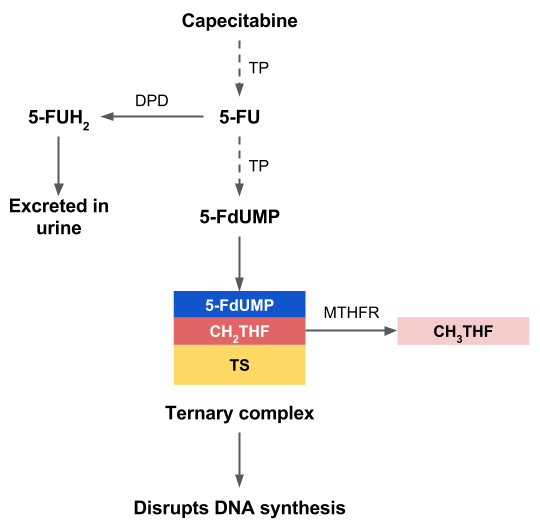
\includegraphics[scale=0.6]{fluorouracil.png}
	\caption[Involvement of TS, DPD, TP, and MTHFR in 5-FU mechanism of action.]{Involvement of TS, DPD, TP, and MTHFR in 5-FU mechanism of action. Dashed lines indicate more than one process is involved in producing the output, whereas solid lines indicate direct reactions. 5-FU, fluorouracil; 5-FdUMP, fluorodeoxyuridine monophosphate; 5-FUH\textsubscript{2}, dihydrofluorouracil; CH\textsubscript{2}THF, 5,10-methylenetetrahydrofolate; CH\textsubscript{3}THF, 5-methyltetrahydrofolate.}
	\label{fig:fluorouracil}
\end{figure}

%%%%%%%%%%%%%%%%%%%%%%%%%%%%%%%%%%%%%%%%%%%%%%%%%%%%%%%%%%%%%%%%%%%%%
%%%%%%%%%%%%%%%%%%%%%%%%%%%%%%%%%%%%%%%%%%%%%%%%%%%%%%%%%%%%%%%%%%%%%

\vspace{5mm}
\noindent\textit{Oxaliplatin}

Oxaliplatin is a platinum derivative commonly used in combination with 5-FU for treating gastric and colorectal cancers. Deactivation of oxaliplatin can be induced by conjugation of the platinum derivative with glutathione (GSH), which is catalyzed by glutathione S-transferases (\acs{GSTP}). While there are studies suggesting that germline variants in the \acs{GSTP1} gene are associated with increased neurotoxicity in patients treated with oxaliplatin combination therapy, there are also groups reporting conflicting results. Therefore, additional studies are required to confirm the impact of \textit{GSTP1} polymorphisms on oxaliplatin treatment \cite{Panczyk2014, Mohelnikova-Duchonova2014}.

\newpage
\vspace{5mm}
\noindent\textit{Irinotecan}

Irinotecan is a camptothecin analog widely used in chemotherapy regimens for treating lung cancers and CRC. The active metabolite of irinotecan, SN-38, blocks type I DNA topoisomerase, impairing DNA replication. SN-38 is inactivated in the liver by uridine diphosphate glycosyltransferase 1 family enzymes (\acs{UGT1A}) through glucuronidation and then excreted. Thus, patients with deficiency in UGT1A, which can be caused by germline variants in the \acs{UGT1A1} gene, are at higher risk of experiencing toxicity due to a longer half-life of SN-38. An example of a germline variant in \textit{UGT1A1} that results in reduced activity is the UGT1A1*28 allele, which corresponds to an extra TA repeat within position -53 and -42 of the translational start codon. Dose reduction is recommended for carriers to prevent toxic effects induced by irinotecan \cite{Panczyk2014, Mohelnikova-Duchonova2014}.

%%%%%%%%%%%%%%%%%%%%%%%%%%%%%%%%%%%%%%%%%%%%%%%%%%%%%%%%%%%%%%%%%%%%%%
\section{Technical challenges in implementing germline testing in clinical oncology}
\label{sec:Challengesinclinicalgermlinetesting}

\subsection{Tumour-only sequencing}

One of the challenges in integrating germline testing in clinical oncology is tumours are often sequenced without matched normal samples. Although sequencing of matched normal samples would allow accurate identification of somatic mutations and simultaneous detection of clinically important germline variants, it is common for clinical laboratories to only sequence tumour samples to minimize cost and turnaround time. However, genomic analyses of tumours can reveal clinically relevant germline variants \cite{Schrader2015, Jones2015a, Meric-Bernstam2016, Bombard2014, WcWhinney2009}. For examples, Schrader et al. \cite{Schrader2015} reported that pathogenic germline variants in CPGs were retained in the tumour genomes of 91.9\% of patients in the study cohort. Hence, clinical laboratories could leverage tumour genomic testing for identification of germline variants and subsequently refer potential germline variants to downstream confirmatory testing.

A clinical pipeline that leverages tumour genomic testing to perform initial screening for germline alterations could provide germline testing in a cost-effective manner because only selected patients would require follow-up testing. However, as the tumour genome contains both germline and somatic variants, the difficulty remains in devising an approach to accurately separate germline variants from somatic mutations. Jones et al. \cite{Jones2015a} used public databases like \acs{dbSNP} and \acs{COSMIC}, as well as effect prediction tool to distinguish between germline and somatic variants, but reported high false positive rates. The use of these public databases cannot reliably differentiate between variant statuses because it is possible for a germline variant to occur somatically, and \textit{vice versa}. For instance, an evaluation of 468 genes with known somatic driver mutations recorded in the COSMIC database showed that 49 of these genes were also known to harbour germline alterations that are associated with inherited predisposition to cancer \cite{Rahman2014}.

One possible approach is the use of VAF to discriminate between germline and somatic variants. Because tumour biopsies are typically admixtures of tumour and normal cells, there is a high likelihood that somatic mutations might deviate from diploid zygosity (i.e. heterozygous variants are expected to have VAF close to 50\%, whereas homozygous variants are expected to have VAF close to 100\%; \autoref{fig:vaf_cells}A). Moreover, tumour heterogeneity might also give rise to VAF deviations (\autoref{fig:vaf_cells}B). Therefore, the use of VAF threshold could be a potential solution in distinguishing between germline and somatic alterations in genomic analyses of tumours without matched normal DNA.

%%%%%%%%%%%%%%%%%%%%%%%%%%%%%%%%%%%%%%%%%%%%%%%%%%%%%%%%%%%%%%%%%%%%%
%%%%%%%%%%%%%%%%%%%%%%%%%%%%%%%%%%%%%%%%%%%%%%%%%%%%%%%%%%%%%%%%%%%%%

\begin{figure}[H]
	\centering
	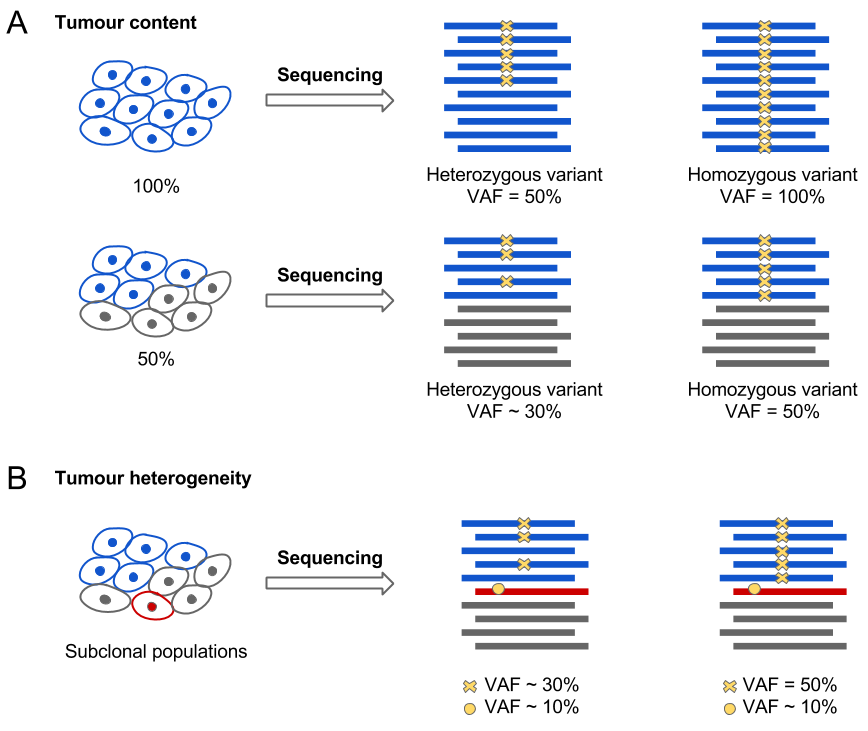
\includegraphics[scale=0.5]{vaf_cells.png}
	\caption[Deviations of VAF as a result of tumour content and heterogeneity.]{Deviations of VAF as a result of tumour content and heterogeneity. Blue and red cells represent tumour cells, whereas grey cells represent normal cells.}
	\label{fig:vaf_cells}
\end{figure}

%%%%%%%%%%%%%%%%%%%%%%%%%%%%%%%%%%%%%%%%%%%%%%%%%%%%%%%%%%%%%%%%%%%%%
%%%%%%%%%%%%%%%%%%%%%%%%%%%%%%%%%%%%%%%%%%%%%%%%%%%%%%%%%%%%%%%%%%%%%

\subsection{Formalin-fixed paraffin-embedded tumours}

Another disadvantage of performing germline variant analysis using tumour DNA is tumour samples in the clinic are often formalin-fixed paraffin-embedded (\acs{FFPE}). Formalin fixation preserves tissue morphology for histological assessment, whereas paraffin embedding enables stable storage of specimens at room temperature, which is cost- and space-saving compared to maintaining fresh frozen specimens in freezers \cite{Dong2015, Do2015a}. DNA isolated from FFPE tumours pose technical challenges in molecular testing because formalin fixation induces several types of DNA damage \cite{Do2015a}. Therefore, assessment of these different forms of DNA damage is essential to establish quality control for a clinical genomic assay.

The main component of formalin, formaldehyde, can react with DNA bases and proteins, producing DNA-DNA, DNA-protein, and protein-protein crosslinks. Additionally, formaldehyde-DNA adducts can also be generated in formalin-fixed tissues. Crosslinking induced by formaldehyde destabilizes the DNA structure, resulting in degradation and low DNA yields extracted from FFPE tissues \cite{Do2015a}. Another predominant form of formalin-induced DNA damage is DNA fragmentation. Hence, FFPE tissues not only produce low quantities of DNA, but also DNA with short fragment sizes. Particularly, this interferes with amplicon-based methods by reducing the amount of amplifiable DNA templates \cite{Shi2002, Didelot2013, Wong2013}. Severity of DNA fragmentation also increases with age of paraffin blocks and acidity of formalin solution used in tissue fixation \cite{Ludyga2012, Carrick2015}.

FFPE DNA also constitutes increased frequency of sequence artifacts. This is problematic in clinical practice because there is a high risk of misinterpreting artifactual base changes as true mutations that may influence patient care. Oxidization of formaldehyde, which generates formic acid, creates an acidic environment that catalyzes hydrolytic cleavage of \textit{N}-glycosidic bonds between purines and the sugar backbone \cite{Do2015a}. This produces abasic sites at which sequence artifacts can occur as most DNA polymerases tend to selectively incorporate adenines across abasic sites during the extension stage. In fewer cases, guanines and short deletions ranging from 1--3 bases could also be introduced by DNA polymerase when synthesizing through abasic sites \cite{Heyn2010}.

A well-documented source of sequence artifacts in FFPE DNA is cytosine deamination. This generates uracil lesions, which leads to artifactual C$>$T/G$>$A transitions because thymines are added opposite of uracils during synthesis of complementary DNA strands \cite{Do2015a}. Wong et al. \cite{Wong2014} showed increased levels of C$>$T/G$>$A artifacts in amplicon sequencing data generated from highly fragmented DNA samples. This observation was attributed to a higher probability of amplifying DNA templates containing sequence artifacts in samples with reduced amount of amplifiable DNA templates as a result of fragmentation damage \cite{Wong2014}. While cytosines can be restored by treating FFPE DNA with uracil-DNA glycosylase (\acs{UDG}) to eliminate uracil lesions, there is currently no method to repair deamination of 5-methylcytosine (5-mC). 5-mC are common at CpG dinucleotides and are more susceptible to deamination in formalin-fixed tissues. Deamination of 5-mC gives rise to thymine instead of uracil, thus cannot be reinstated through treatment with the UDG enzyme \cite{Do2015a}.

%%%%%%%%%%%%%%%%%%%%%%%%%%%%%%%%%%%%%%%%%%%%%%%%%%%%%%%%%%%%%%%%%%%%%%
\section{Objectives}
\label{sec:Objectives}

Germline alterations have clinical implications for cancer patients and their family members. Because the tumour genome contains both somatic and germline variants, clinical tumour sequencing presents an opportunity for pre-screening of germline variants. This framework is a time- and cost-effective approach for providing germline testing because only patients with potential germline variants would require downstream confirmatory testing. A primary challenge in implementing this framework for identifying clinically significant germline variants is differentiating between germline and somatic alterations in the tumour genome. Tumour specimens also tend to be FFPE, which causes DNA damage that could affect the use of FFPE DNA for clinical genomic testing.

To date, no study has evaluated the detection of germline alterations in FFPE tumours using NGS-based tests. As formalin fixation is known to cause DNA damage, the usability of FFPE DNA for NGS-based germline testing must be compared to a gold standard such as blood DNA. To determine reliability of using tumour DNA for germline variant calling, retention rate of germline variants in the tumour genome must be measured. This is because tumour-specific mutations might result in loss of germline variants. Currently, there is also no standard method in distinguishing between germline and somatic variants in tumour-only analyses. Hence, an approach to distinguish between germline and somatic variants in tumour genomes must be established and assessed for its sensitivity and precision.

In this study, we aimed to determine whether potential germline alterations can be accurately identified through genomic analyses of FFPE tumours. We performed analytic validation of a clinical amplicon-based targeted sequencing panel for FFPE solid tumours by comparison with sequencing of blood DNA, which is the gold standard for germline testing. We identified three objectives in this study:

\begin{enumerate}
\item Assess the degree of formalin-induced DNA damage in FFPE DNA
\item Determine the retention rate of germline alterations in FFPE tumours, and
\item Evaluate the use of VAF thresholds to distinguish germline alterations from somatic mutations in tumour-only analyses.
\end{enumerate}

\noindent{Through these analyses, we hoped to characterize formalin-induced DNA damage to facilitate quality control and improve robustness of our assay. Finally, we also aimed to measure the sensitivities for identifying potential germline alterations and positive predictive values (PPVs) for referring germline alterations to downstream germline testing at various VAF cut-offs. Establishing these performance parameters would serve as important guidelines in clinical practice.}

%%%%%%%%%%%%%%%%%%%%%%%%%%%%%%%%%%%%%%%%%%%%%%%%%%%%%%%%%%%%%%%%%%%%%%
\endinput


Both von Hansemann and Boveri observed unequal chromosomal segregations in tumour cells, which prompted their speculations that tumour development is induced by anomalies in hereditary material \cite{VonHansemann1890, Boveri1914}. An observation that drew Boveri's attention is that not all chromosomal imbalanced cells proliferated uncontrollably and formed tumours, there were some that resulted in cell death. This led Boveri to further hypothesize that genetic materials are functionally different, and tumour formation is promoted by retention of chromatin parts that stimulate growth or elimination of those that inhibit growth, concepts that manifested in the present knowledge of oncogenes and tumour-suppressor genes, respectively \cite{Boveri1914}.

Clinical targeted panels can also differ based on testing content, which can be limited to cancer hotspots. The Illumina TruSeq Amplicon Cancer Panel (TSACP) is an example of a commercially available hotspot panel that surveys frequently mutated sites in 48 genes using 212 amplicons. These genes include \textit{BRAF}, \textit{KRAS}, and \textit{EGFR}, which have clinical implications for various cancers like melanoma, and colorectal and lung cancers. For example, somatic mutations in codon 12 and 13 of \textit{KRAS} such as pG12V, pG12D, and pG13D, are known negative predictors for response to anti-EGFR monoclonal antibody therapies. These cancer hotspots are recommended for molecular testing in colorectal cancer patients by an expert panel put together by the American Society for Clinical Pathology (ASCP), College of American Pathologists (CAP), Association for Molecular Pathology (AMP), and the American Society of Clinical Oncology (ASCO). Using the TSACP to sequence formalin-fixed paraffin-embedded (FFPE) colon tumours, Simen et al. \cite{} reported hotspot mutations in codon 12 and 13 of \textit{KRAS} and exons 18 to 21 of \textit{EGFR}, as well as BRAF V600E mutations, and performed further validation using Sanger sequencing, which demonstrated 100\% concordance. Further validation also showed that results were 100\% concordant with Sanger sequencing. Somatic mutations

%%%%%%%%%%%%%%%%%%%%%%%%%%%%%%%%%%%%%%%%%%%%%%%%%%%%%%%%%%%%%%%%%%%%%%
\section{Cancer as a Genetic Disease}
\label{sec:CancerasaGeneticDisease}

Cancers are diseases defined by unrestrained proliferation of cells that are capable of invading normal tissues and metastasizing to other parts of the body. Early studies between the late nineteenth and early twentieth centuries by David von Hansemann and Theodor Boveri suggested that genetic alterations may contribute to oncogenesis. In von Hansemann's analysis of tumour samples, he observed features of aberrant cell division, which he speculated to be contributing factors of unequal distribution of chromosomes in the tumour cells. Boveri explored the connection between defective cell division and tumour formation by inducing abnormal chromosome segregation in sea urchin eggs and observing the outcome of these cells. While most cases of chromosomal imbalance resulted in cell death, Boveri reported that there were cases in which cell survival was followed by uncontrolled cell growth. These findings led Boveri to surmise that the improper combination of genetic materials could sustain the proliferative ability of tumour cells. In particular, tumour cells were likely to retain chromatin parts with growth stimulatory effects or remove those with growth inhibitory effects. Boveri's speculations pertaining genetic materials that function as stimulators or inhibitors of cell growth were consistent with the modern understanding of oncogenes and tumour-suppressor genes, respectively.

Oncogenes and tumour-suppressor genes are two categories of cancer-causing genes that play a central role in cancer initiation and progression. Prototype oncogenes (proto-oncogenes), the normal counterparts of oncogenes, encode proteins that promote cell growth and survival, as well as inhibit cell differentiation. When proto-oncogenes sustain dominant gain-of-function mutations, they become oncogenes, giving rise to constitutively active or overexpressed protein products that induce malignant transformation of the cells. The first oncogene, v-\textit{src}, was identified by Peyton Rous in a retrovirus that causes sarcoma in chickens, and the virus was later named the Rous sarcoma virus after its discoverer. Subsequently, the proto-oncogene c-\textit{src}, a homologue of v-\textit{src}, was discovered, but unlike its mutant form, the protein encoded by c-\textit{src} was not constitutively active. The discovery that proto-oncogenes exist in healthy cells led to the recognition that normal cellular genes are capable of gaining oncogenic potential through acquiring gene mutations. This breakthrough in cancer research consequently catalyzed the identification of more proto-oncogenes, providing an enhanced understanding of cellular signalling pathways.

Tumour-suppressor genes, the other important type of cancer-causing genes, can be separated into gatekeepers and caretakers. Gatekeepers are involved in regulating cell-cycle checkpoints and mutations in gatekeepers would directly result in cancer development. On the other hand, caretakers are DNA repair proteins, and mutant caretakers could indirectly cause malignant transformation of cells by inducing accumulation of mutations, thereby increasing the probability that mutations would occur in oncogenes and tumour-suppressor genes. Unlike oncogenes, mutations in tumour-suppressor genes are recessive-acting, meaning that two mutant alleles are required for the tumour-suppressor gene to become oncogenic. Alfred Knudson was the first to propose that mutant tumor-suppressor genes function in a recessive fashion, a notable concept later known as Knudson's two-hit hypothesis.  Knudson's statistical model demonstrated that familial retinoblastoma, a pediatric eye cancer, was consistent with a one-hit curve, meaning that a single mutation was sufficient to cause tumour formation. Conversely, non-familial retinoblastoma was consistent with a two-hit curve, meaning that two mutations were involved in the disease. These findings implied that disease carriers, who inherited one mutant allele, only require the loss of the remaining functional allele to drive tumour formation, whereas non-carriers require two mutation events to trigger the development of tumours.

Some bullshit about stepwise progression...

%%%%%%%%%%%%%%%%%%%%%%%%%%%%%%%%%%%%%%%%%%%%%%%%%%%%%%%%%%%%%%%%%%%%%%
\section{The Evolution of Molecular Diagnostics in Cancer}
\label{sec:The Evolution of Molecular Diagnostics in Cancer}

Although early studies have implicated the causative role of genetic alterations in cancer development, initial classification of cancers were based on the primary site of the tumour. This long-standing classification was caused by limitations in technologies and tools, as well as by the clinical classification required by surgical management, which was the initial mainstay of clinical oncology. Subsequently, microscopy-based classification of disease further delineated cancer subsets based on histologic differences. For example, aggressiveness or risk of relapse was retrospectively linked to histologic grading as a prognostic biomarker, such as Gleason and Bloom-Richardson for prostate and breast cancer, respectively. The histologic classification was advanced with assessment of prototypic surface markers (immunohistochemistry), gross markers for lymphoid subsets have heavily influenced the diagnostic classification of lymphoma. Characterization of chromosomal abnormalities in leukemia and sarcoma has aided in the diagnosis of disease subsets as well as prognostic assessment.

In conclusion, the diagnosis of cancer has undergone a paradigm shift. No longer is cancer diagnosed only based on morphological parameters. More and more the diagnostic algorithm is supported by immunohistochemical and molecular alterations at the DNA, mRNAs, miRNAs and proteomic level. Multiple platforms and high throughput technological advances enable faster and cheaper analysis of all these as well as the whole genome. This is having a significant impact on how medicine is now being practiced in a personalized approach leading to the development of precision medicine based on pharmacogenomics. It is being realized that a tumor may not be characterized by a single gene alteration but by a panel of ‘signature’ genomic alterations leading to targeted therapeutic strategies and surveillance based on the tumor specific alterations. The ultimate goal of cancer diagnosis in personalized medicine would be to identify the correct diagnosis and guide the therapy so that every patient received precision medicine that is the right drug at the right dose.

Cancer is a group of diseases characterized by uncontrolled proliferation of cells that are capable of normal tissue invasion and metastasis to distant organs.

Oncogenes encode for proteins that stimulate cell proliferation and survival as well as inhibit cell differentiation leading to oncogenesis. The first human oncogene was identified based on homology with

Mutations in oncogenes are typically dominant, which means . The first human oncogenes was discovered Conversely, tumour-suppressor genes encode for proteins that inhibit cell proliferation and survival as well as stimulate cell differentiation. Mutations in oncogenes are typically dominant whereas mutations in tumour-suppressor genes are recessive.

In the normal cell, proto-oncogenes stimulate proliferation and inhibit differentiation and apoptosis while the opposite is true for tumour suppressors. Proto-oncogenes are usually dominant, meaning that only one gain-of-function mutation is required to activate the oncogene, thereby causing cancer. Conversely, tumour suppressor genes are usually recessive and two loss-of-function events are required.

Boveri and von Hansemann (1890-1914) - oncogenes and tumour suppressors
Philadelphia translocation (1960)
Two hit hypothesis, retinoblastoma (1971) - germline and somatic mutations
HRAS point mutation (1982)
Eric Fearon and Bert Vogelstein find specific sequential mutations in carcinoma (1990) - multi-step process, caretakers and gatekeepers
Types of mutations/gene changes - SNVs, indels, SVs
Driver vs. passenger mutations - evolutionary process, selective growth advantage, CSCs
Frequency and pathway-based: three main pathways

The pathogenesis of cancer is caused by genetic abnormalities
Although fundamentally known to arise from genetic mutations, the disease paradigm has expanded to include aberrant epigenetic mechanisms as a contributing factor to oncogenesis.
The understanding of cancer pathogenesis has expanded been increasing over the years and a disorder that was fundamentally known to arise from genetic mutations this group of disorders which have been fundamentally known Cancer has been fundamentally known as a genetic disease defined by abnormal proliferation of cells.
Our understanding of cancer pathogenesis has been expanding  Although the understanding of cancer pathogenesis has been expanding, Cancer has been fundamentally known as a genetic disease.
